\section{About Dataset}

We use the Breast Cancer Wisconsin (Diagnostic) Data Set from Kaggle found \href{https://www.kaggle.com/datasets/uciml/breast-cancer-wisconsin-data}{here}.
The dataset contains 569 rows with 33 attributes.

The attribute we analyze is \textit{perimeter\_mean}, which is the mean size of the core tumor.
Refer to \autoref{fig:hist} for the histogram of this attribute.

\begin{figure}[!ht]
  \centering
  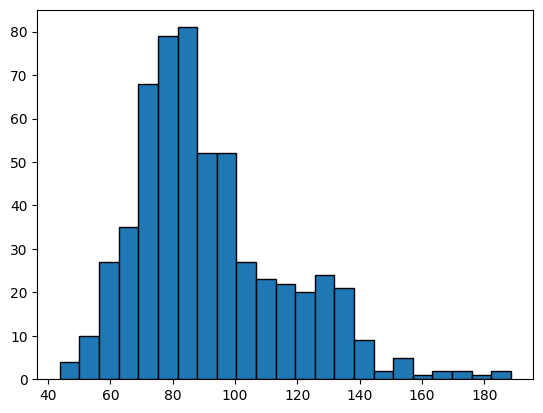
\includegraphics[width=.5\textwidth]{images/data-hist.png}
  \caption{Histogram of the attribute perimeter\_mean}
  \label{fig:hist}
\end{figure}
